
\begin{center}
    \textbf{Equilibro general}
\end{center}

\begin{center}
\textbf{Prof. Carlos Hervés Beloso}
\end{center}

\begin{center}
\textbf{Alumno: Christian Limbert Paredes Aguilera}
\end{center}

\begin{center}
	\rule{0.5\textwidth}{0.4pt}
\end{center}
\vspace{1cm}

\begin{enumerate}[\textbf{Ejercicio} \bfseries 1.]

    %-------------------- 1.
    \item \textbf{\boldmath Represente la caja de Edgeworth para una economía con dos bienes $(x_1,x_2)$ y dos agentes $(j,k)$, donde las dotaciones iniciales son $\omega_j=(15,10)$ y $\omega_k=(5,10)$.}\\

	\textbf{Solución:}\;
	\begin{center}
	    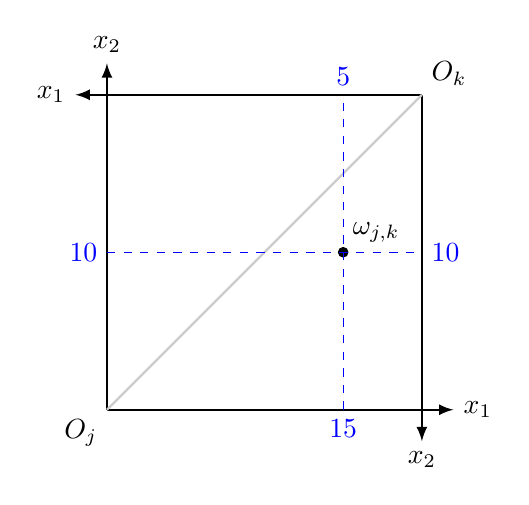
\begin{tikzpicture}[scale=0.2]
		\coordinate (A) at (0,0);
		\coordinate (B) at (20,20);
		\begin{scope}[->,>=latex,thick]
		    \draw (A) -- +(22,0)node[right]{$x_1$};
		    \draw (A) -- +(0,22)node[above]{$x_2$};
		    \draw (B) -- +(-22,0)node[left]{$x_1$};
		    \draw (B) -- +(0,-22)node[below]{$x_2$};
		\end{scope}
		\node[below left] at (A) {$O_j$};
		\node[above right] at (B) {$O_k$};

		\draw[fill=black] (15,10) circle (0.3cm) node[above right]{$\omega_{j,k}$};

		\draw[thick,gray!40] (0,0) -- (20,20);

		\draw[dashed,blue] (0,10)node[left]{$10$} -- (20,10)node[right]{$10$};
		\draw[dashed,blue] (15,0)node[below]{$15$} -- (15,20)node[above]{$5$};
	    \end{tikzpicture}
	\end{center}

    %-------------------- 2.
    \item \textbf{\boldmath Asumiendo las dotaciones del ejercicio anterior, describa gráficamente todas las asignaciones Pareto eficientes para cada uno de los siguientes casos. Explique brevemente la forma de todas ellas en relación a las preferencias de los individuos.}

	\begin{enumerate}[\bfseries i)]

	    %---------- i)
	    \item \textbf{\boldmath $u_j(x_1,x_2)=2x_1+x_2$; $u_k(x_1,x_2)=x_1+2x_2$.}\\

		\textbf{Solución:}\;
		\begin{center}
		    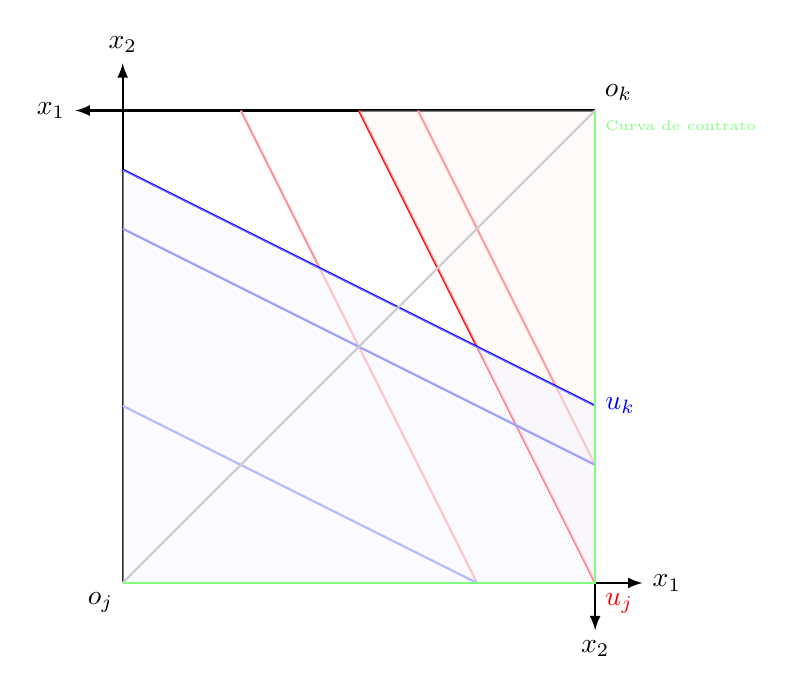
\begin{tikzpicture}[scale=0.3]
			\coordinate (a) at (0,0);
			\coordinate (b) at (20,20);
			\begin{scope}[->,>=latex,thick]
			\draw (a) -- +(22,0)node[right]{$x_1$};
			\draw (a) -- +(0,22)node[above]{$x_2$};
			\draw (b) -- +(-22,0)node[left]{$x_1$};
			\draw (b) -- +(0,-22)node[below]{$x_2$};
			\end{scope}
			\node[below left] at (a) {$o_j$};
			\node[above right] at (b) {$o_k$};

			% curvas de indiferencia
			%\draw[variable=\x,domain=0:2.5,thick,red!40] plot ({\x},{5-2*\x});
			%\draw[variable=\x,domain=0:5,thick,red!40] plot ({\x},{10-2*\x});
			%\draw[variable=\x,domain=0:7.5,thick,red!40] plot ({\x},{15-2*\x});
			%\draw[variable=\x,domain=0:10,thick,red!40] plot ({\x},{20-2*\x});
			%\draw[variable=\x,domain=2.5:12.5,thick,red!40] plot ({\x},{25-2*\x});
			\draw[variable=\x,domain=5:15,thick,red!40] plot ({\x},{30-2*\x});
			%\draw[variable=\x,domain=7.5:17.5,thick,red!40] plot ({\x},{35-2*\x});
			\draw[variable=\x,domain=10:20,thick,red] plot ({\x},{40-2*\x})node[below right]{$u_j$};
			\draw[variable=\x,domain=12.5:20,thick,red!70] plot ({\x},{45-2*\x});
			%\draw[variable=\x,domain=15:20,thick,red!40] plot ({\x},{50-2*\x});
			%\draw[variable=\x,domain=17.5:20,thick,red!40] plot ({\x},{55-2*\x});
			\fill[fill=red!4,opacity=.5] (10,20) -- plot[domain=10:20] (\x,{40-2*\x}) -- (20,20);

			%\draw[variable=\x,domain=0:5,thick,blue!50] plot ({\x},{(5-\x)/2});
			%\draw[variable=\x,domain=0:10,thick,blue!50] plot ({\x},{(10-\x)/2});
			\draw[variable=\x,domain=0:15,thick,blue!50] plot ({\x},{(15-\x)/2});
			%\draw[variable=\x,domain=0:20,thick,blue!50] plot ({\x},{(20-\x)/2});
			%\draw[variable=\x,domain=0:20,thick,blue!50] plot ({\x},{(25-\x)/2});
			\draw[variable=\x,domain=0:20,thick,blue!70] plot ({\x},{(30-\x)/2});
			\draw[variable=\x,domain=0:20,thick,blue] plot ({\x},{(35-\x)/2})node[right]{$u_k$};
			%\draw[variable=\x,domain=0:20,thick,blue!50] plot ({\x},{(40-\x)/2});
			%\draw[variable=\x,domain=5:20,thick,blue!50] plot ({\x},{(45-\x)/2});
			%\draw[variable=\x,domain=10:20,thick,blue!50] plot ({\x},{(50-\x)/2});
			%\draw[variable=\x,domain=15:20,thick,blue!50] plot ({\x},{(55-\x)/2});
			\fill[fill=blue!4,opacity=.5] (0,0) -- plot[domain=0:20] (\x,{(35-\x)/2}) -- (20,0);

			% curva de contrato
			\draw[thick,green!50] (0,0)--(20,0)--(20,20)node[below right]{\tiny Curva de contrato};

			\draw[thick,gray!40] (0,0) -- (20,20);
		    \end{tikzpicture}
		\end{center}


	    %---------- ii)
	    \item \textbf{\boldmath $u_j(x_1,x_2)=u_k(x_1,x_2)=x_1+x_2$.}\\

		\textbf{Solución:}
		\begin{center}
		    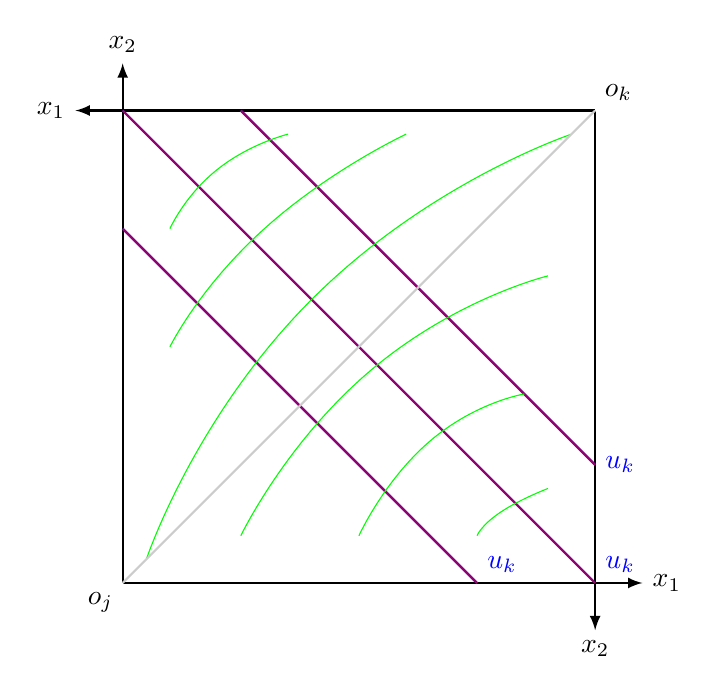
\begin{tikzpicture}[scale=0.3]
			\coordinate (a) at (0,0);
			\coordinate (b) at (20,20);
			\begin{scope}[->,>=latex,thick]
			\draw (a) -- +(22,0)node[right]{$x_1$};
			\draw (a) -- +(0,22)node[above]{$x_2$};
			\draw (b) -- +(-22,0)node[left]{$x_1$};
			\draw (b) -- +(0,-22)node[below]{$x_2$};
			\end{scope}
			\node[below left] at (a) {$o_j$};
			\node[above right] at (b) {$o_k$};

			% curvas de indiferencia
			\draw[variable=\x,domain=5:20,thick,blue] plot ({\x},{25-\x})node[right]{$u_k$};
			\draw[variable=\x,domain=5:20,thick,red,opacity=.6] plot ({\x},{25-\x});

			\draw[variable=\x,domain=0:20,thick,blue] plot ({\x},{20-\x})node[above right]{$u_k$};
			\draw[variable=\x,domain=0:20,thick,red,opacity=.6] plot ({\x},{20-\x});

			\draw[variable=\x,domain=0:15,thick,blue] plot ({\x},{15-\x})node[above right]{$u_k$};
			\draw[variable=\x,domain=0:15,thick,red,opacity=.6] plot ({\x},{15-\x});

			% curva de contrato
			\draw[green] plot [smooth, tension=1] coordinates {(2,15) (4,17.5) (7,19)};
			\draw[green] plot [smooth, tension=1] coordinates {(2,10) (6,15) (12,19)};
			\draw[green] plot [smooth, tension=1] coordinates {(1,1) (8,12) (19,19)};
			\draw[green] plot [smooth, tension=1] coordinates {(5,2) (10.5,9) (18,13)};
			\draw[green] plot [smooth, tension=1] coordinates {(10,2) (13,6) (17,8)};
			\draw[green] plot [smooth, tension=1] coordinates {(15,2) (16,3) (18,4)};

			\draw[thick,gray!40] (0,0) -- (20,20);
		    \end{tikzpicture}
		\end{center}


	    %---------- iii)
	    \item \textbf{\boldmath $u_j(x_1,x_2)=x_1+4x_2$; $u_k(x_1,x_2)=x_1+2x_2$.}\\

		\textbf{Solución:}
		\begin{center}
		    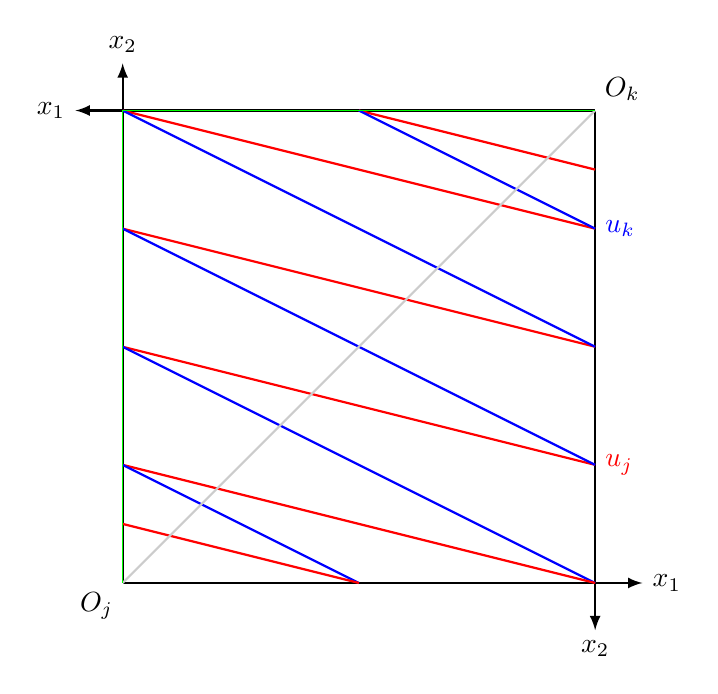
\begin{tikzpicture}[scale=0.3]
			\coordinate (A) at (0,0);
			\coordinate (B) at (20,20);
			\begin{scope}[->,>=latex,thick]
			    \draw (A) -- +(22,0)node[right]{$x_1$};
			    \draw (A) -- +(0,22)node[above]{$x_2$};
			    \draw (B) -- +(-22,0)node[left]{$x_1$};
			    \draw (B) -- +(0,-22)node[below]{$x_2$};
			\end{scope}
			\node[below left] at (A) {$O_j$};
			\node[above right] at (B) {$O_k$};


			\draw[red,variable=\x,domain=10:20,thick] plot ({\x},{(90-\x)/4});

			\draw[red,variable=\x,domain=0:20,thick] plot ({\x},{(80-\x)/4});

			\draw[red,variable=\x,domain=0:20,thick] plot ({\x},{(60-\x)/4});

			\draw[blue,variable=\x,domain=10:20,thick] plot ({\x},{(50-\x)/2})node[right]{$u_k$};


			\draw[blue,variable=\x,domain=0:20,thick] plot ({\x},{(40-\x)/2});
			\draw[red,variable=\x,domain=0:20,thick] plot ({\x},{(40-\x)/4})node[right]{$u_j$};

			\draw[blue,variable=\x,domain=0:20,thick] plot ({\x},{(30-\x)/2});

			\draw[blue,variable=\x,domain=0:20,thick] plot ({\x},{(20-\x)/2});
			\draw[red,variable=\x,domain=0:20,thick] plot ({\x},{(20-\x)/4});

			\draw[blue,variable=\x,domain=0:10,thick] plot ({\x},{(10-\x)/2});
			\draw[red,variable=\x,domain=0:10,thick] plot ({\x},{(10-\x)/4});

			\draw[thick,gray!40] (0,0) -- (20,20);


			\draw[green](20,20)--(0,20)--(0,0);
		    \end{tikzpicture}
		\end{center}
\newpage
	    %---------- iv)
	    \item \textbf{\boldmath $u_j(x_1,x_2)=u_k(x_1,x_2)=\min\left\{x_1;x_2\right\}$.}\\

		\textbf{Solución:}
		\begin{center}
		    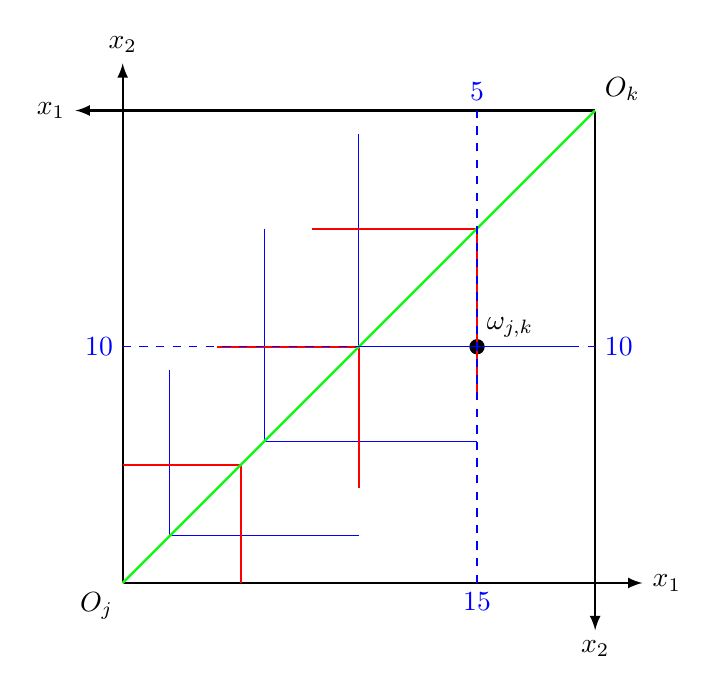
\begin{tikzpicture}[scale=0.3]
			\coordinate (A) at (0,0);
			\coordinate (B) at (20,20);
			\begin{scope}[->,>=latex,thick]
			    \draw (A) -- +(22,0)node[right]{$x_1$};
			    \draw (A) -- +(0,22)node[above]{$x_2$};
			    \draw (B) -- +(-22,0)node[left]{$x_1$};
			    \draw (B) -- +(0,-22)node[below]{$x_2$};
			\end{scope}
			\node[below left] at (A) {$O_j$};
			\node[above right] at (B) {$O_k$};

			\draw[fill=black] (15,10) circle (0.3cm) node[above right]{$\omega_{j,k}$};

			\draw[blue](10,19)--(10,10)--(19,10);
			\draw[blue](6,15)--(6,6)--(15,6);
			\draw[blue](2,9)--(2,2)--(10,2);

			\draw[thick,red](8,15)--(15,15)--(15,8);
			\draw[thick,red](4,10)--(10,10)--(10,4);
			\draw[thick,red](0,5)--(5,5)--(5,0);

			\draw[thick,gray!40] (0,0) -- (20,20);
			\draw[thick,green] (0,0) -- (20,20);

			\draw[dashed,blue] (0,10)node[left]{$10$} -- (20,10)node[right]{$10$};
			\draw[dashed,blue] (15,0)node[below]{$15$} -- (15,20)node[above]{$5$};
		    \end{tikzpicture}
		\end{center}

	    %---------- v)
	    \item \textbf{\boldmath $u_j(x_1,x_2)=u_k(x_1,x_2)=\min\left\{\frac{x_1}{2};x_2\right\}$.}\\

		\textbf{Solución:}
		\begin{center}
		    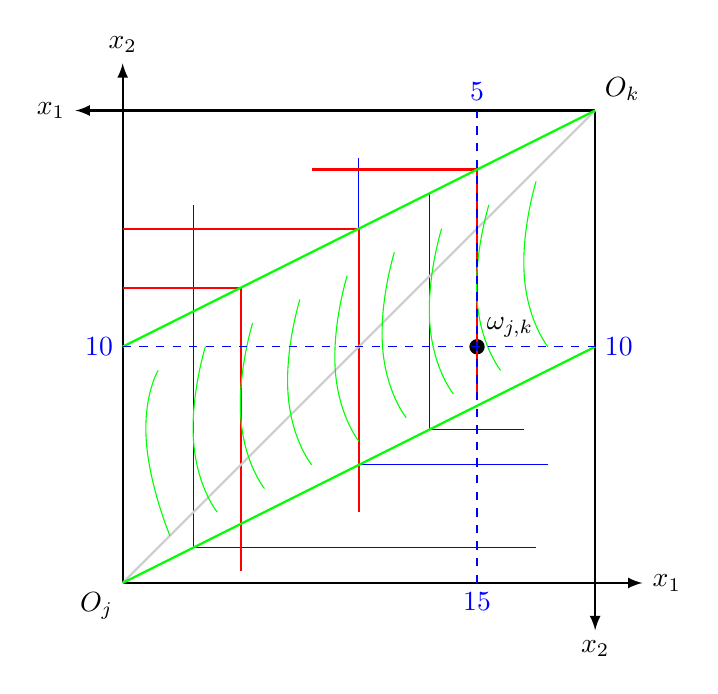
\begin{tikzpicture}[scale=0.3]
			\coordinate (A) at (0,0);
			\coordinate (B) at (20,20);
			\begin{scope}[->,>=latex,thick]
			    \draw (A) -- +(22,0)node[right]{$x_1$};
			    \draw (A) -- +(0,22)node[above]{$x_2$};
			    \draw (B) -- +(-22,0)node[left]{$x_1$};
			    \draw (B) -- +(0,-22)node[below]{$x_2$};
			\end{scope}
			\node[below left] at (A) {$O_j$};
			\node[above right] at (B) {$O_k$};

			\draw[fill=black] (15,10) circle (0.3cm) node[above right]{$\omega_{j,k}$};

			\draw[blue](13,16.5)--(13,6.5)--(17,6.5);
			\draw[blue](10,18)--(10,5)--(18,5);
			\draw[blue](3,16)--(3,1.5)--(17.5,1.5);

			\draw[thick,red](8,17.5)--(15,17.5)--(15,8);
			\draw[thick,red](0,15)--(10,15)--(10,3);
			\draw[thick,red](0,12.5)--(5,12.5)--(5,.5);

			\draw[thick,gray!40] (0,0) -- (20,20);
			\draw[thick,green] (0,10) -- (20,20);
			\draw[thick,green] (0,0) -- (20,10);

			\draw[green] plot [smooth, tension=1] coordinates {(2,2) (1,6) (1.5,9)};
			\draw[green] plot [smooth, tension=1] coordinates {(4,3) (3,6) (3.5,10)};
			\draw[green] plot [smooth, tension=1] coordinates {(6,4) (5,7) (5.5,11)};
			\draw[green] plot [smooth, tension=1] coordinates {(8,5) (7,8) (7.5,12)};
			\draw[green] plot [smooth, tension=1] coordinates {(10,6) (9,9) (9.5,13)};
			\draw[green] plot [smooth, tension=1] coordinates {(12,7) (11,10) (11.5,14)};
			\draw[green] plot [smooth, tension=1] coordinates {(14,8) (13,11) (13.5,15)};
			\draw[green] plot [smooth, tension=1] coordinates {(16,9) (15,12) (15.5,16)};
			\draw[green] plot [smooth, tension=1] coordinates {(18,10) (17,13) (17.5,17)};
			

			\draw[dashed,blue] (0,10)node[left]{$10$} -- (20,10)node[right]{$10$};
			\draw[dashed,blue] (15,0)node[below]{$15$} -- (15,20)node[above]{$5$};
		    \end{tikzpicture}
		\end{center}
\newpage
	    %---------- vi)
	    \item \textbf{\boldmath $u_j(x_1,x_2)=\min\left\{\frac{x_1}{2};x_2\right\}$; $u_k(x_1,x_2)=\min\left\{x_1;\frac{x_2}{2}\right\}$.}\\

		\textbf{Solución:}
		\begin{center}
		    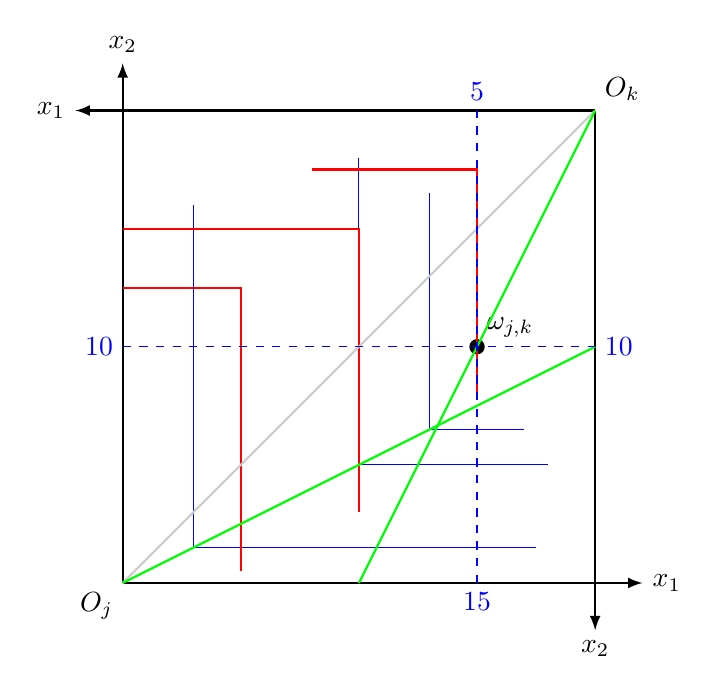
\begin{tikzpicture}[scale=0.3]
			\coordinate (A) at (0,0);
			\coordinate (B) at (20,20);
			\begin{scope}[->,>=latex,thick]
			    \draw (A) -- +(22,0)node[right]{$x_1$};
			    \draw (A) -- +(0,22)node[above]{$x_2$};
			    \draw (B) -- +(-22,0)node[left]{$x_1$};
			    \draw (B) -- +(0,-22)node[below]{$x_2$};
			\end{scope}
			\node[below left] at (A) {$O_j$};
			\node[above right] at (B) {$O_k$};

			\draw[fill=black] (15,10) circle (0.3cm) node[above right]{$\omega_{j,k}$};

			\draw[blue](13,16.5)--(13,6.5)--(17,6.5);
			\draw[blue](10,18)--(10,5)--(18,5);
			\draw[blue](3,16)--(3,1.5)--(17.5,1.5);

			\draw[thick,red](8,17.5)--(15,17.5)--(15,8);
			\draw[thick,red](0,15)--(10,15)--(10,3);
			\draw[thick,red](0,12.5)--(5,12.5)--(5,.5);

			\draw[thick,gray!40] (0,0) -- (20,20);
			\draw[thick,green] (0,0) -- (20,10);
			\draw[thick,green] (20,20) -- (10,0);

			\draw[dashed,blue] (0,10)node[left]{$10$} -- (20,10)node[right]{$10$};
			\draw[dashed,blue] (15,0)node[below]{$15$} -- (15,20)node[above]{$5$};
		    \end{tikzpicture}
		\end{center}

	    %---------- vii)
	    \item \textbf{\boldmath $u_j(x_1,x_2)=u_k(x_1,x_2)=x_1^{1/2}x_2^{1/2}$.}\\

		\textbf{Solución:}
		\begin{center}
		    \begin{tikzpicture}[scale=0.3]
			\coordinate (A) at (0,0);
			\coordinate (B) at (20,20);
			\begin{scope}[->,>=latex,thick]
			    \draw (A) -- +(22,0)node[right]{$x_1$};
			    \draw (A) -- +(0,22)node[above]{$x_2$};
			    \draw (B) -- +(-22,0)node[left]{$x_1$};
			    \draw (B) -- +(0,-22)node[below]{$x_2$};
			\end{scope}
			\node[below left] at (A) {$O_j$};
			\node[above right] at (B) {$O_k$};

			\draw[fill=black] (15,10) circle (0.3cm) node[above right]{$\omega_{j,k}$};

			\draw[thick,gray!40] (0,0) -- (20,20);

			\draw[dashed,blue] (0,10)node[left]{$10$} -- (20,10)node[right]{$10$};
			\draw[dashed,blue] (15,0)node[below]{$15$} -- (15,20)node[above]{$5$};
		    \end{tikzpicture}
		\end{center}

\newpage
	    %---------- viii)
	    \item \textbf{\boldmath $u_j(x_1,x_2)=x_1^{3/2}x_2^{1/4}$; $u_k(x_1,x_2)=x_1^{1/4}x_2^{3/4}$.}\\

		\textbf{Solución:}
		\begin{center}
		    \begin{tikzpicture}[scale=0.3]
			\coordinate (A) at (0,0);
			\coordinate (B) at (20,20);
			\begin{scope}[->,>=latex,thick]
			    \draw (A) -- +(22,0)node[right]{$x_1$};
			    \draw (A) -- +(0,22)node[above]{$x_2$};
			    \draw (B) -- +(-22,0)node[left]{$x_1$};
			    \draw (B) -- +(0,-22)node[below]{$x_2$};
			\end{scope}
			\node[below left] at (A) {$O_j$};
			\node[above right] at (B) {$O_k$};

			\draw[fill=black] (15,10) circle (0.3cm) node[above right]{$\omega_{j,k}$};

			\draw[thick,gray!40] (0,0) -- (20,20);

			\draw[dashed,blue] (0,10)node[left]{$10$} -- (20,10)node[right]{$10$};
			\draw[dashed,blue] (15,0)node[below]{$15$} -- (15,20)node[above]{$5$};
		    \end{tikzpicture}
		\end{center}


	
	\end{enumerate}

\end{enumerate}
